\chapter{Background \& Ojectives}

\section{Background}
\Gls{rts} games have a huge market on desktop environments, but have yet to make the break through into both the console and the mobile gaming markets. This is mostly attributed to the complex control mechanisms that need to be executed precisely. A mobile devices form factor restricts the number of controls that can be presented to the user at any given time as well as the precision in which these commands can be issued.

\Gls{rts} games are generally designed around large, expansive maps that cover a large range of environments and landscapes. The game map shapes how the game will be played, how involved the player feels and ultimately the engagement of players. These maps can take years to develop and result in one of the largest costs within the development process. So when coming up with an environment why not take advantage of a ready made one? That of planet Earth.

Building a game where the game play takes place on a map of Earth has a number of benefits. First is the scale of a map covering 510 million square kilometers of varying terrain and features. This scale also contains a huge level of detail that could not be achieved by a team of designers. Along side this there is the feeling of familiarity, unlike when starting a new game and having to teach the player about the environment, the user will already have a well formed model in their own head. Along with highly detailed knowledge about certain areas especially those within close proximity of their current location.

Mobile devices have a whole host of unique features and sensors that set it apart from other gaming platforms. One feature that has been widely adopted in a huge range of different applications is location. A users location can be easily determined with a number of different components present on most modern smart phones, these are a GPS chip and the mobile GSM network. Although location has been used extensively in applications it has yet to be utilized effectively as a key metric within a game. This extra information about the user would enable a game set around the physical world to be able to be integrated with the user. Instead of placing new users randomly on a unfamiliar map they can be placed in their real location. Thus giving them a chance to use their own knowledge of their surroundings to help them within the game environment.


\section{Market}

A worldwide \gls{rts} game that combines a map of the world and data gathered about the user combine to create a unique gaming experience and could add an entirely new dimension to the genre. This can also reduce the learning curve and thus shorten the time between installation and engagement. With the sheer number of applications available on a mobile platform combined with the ease and minimal to no cost of installing new applications, this is important to reduce the chance of the user simply finding an alternative.

\subsection{Choosing a platform}
The current mobile platform duopoly results in their only being two viable platforms, Apple's iOS and Google's Android OS. The Android operating system, as of February 2013, had over 51\% market share in the US\cite{smartphone_market}. Closely followed by the original and most established app ecosystem of Apple iOS. Even though there are other platforms, such as Windows phone and Blackberry, none of these have the market share allow them to be a primary platform of choice. Therefore choosing between the two platforms can be an important decision for mobile developers, both platforms offer their own unique advantages and disadvantages. Android on the one hand has the lead on market share offering a larger audience, although this will not directly affect engagement or return.

This years Developer Economics report\cite{de} looks at all aspects of the mobile app market and is an invaluable insight into both the market and consumer trends. As well as evaluating the current market it also gets feedback from developers as to their experiences with different platforms as well as their success.

\begin{figure}[H]
  \centering
   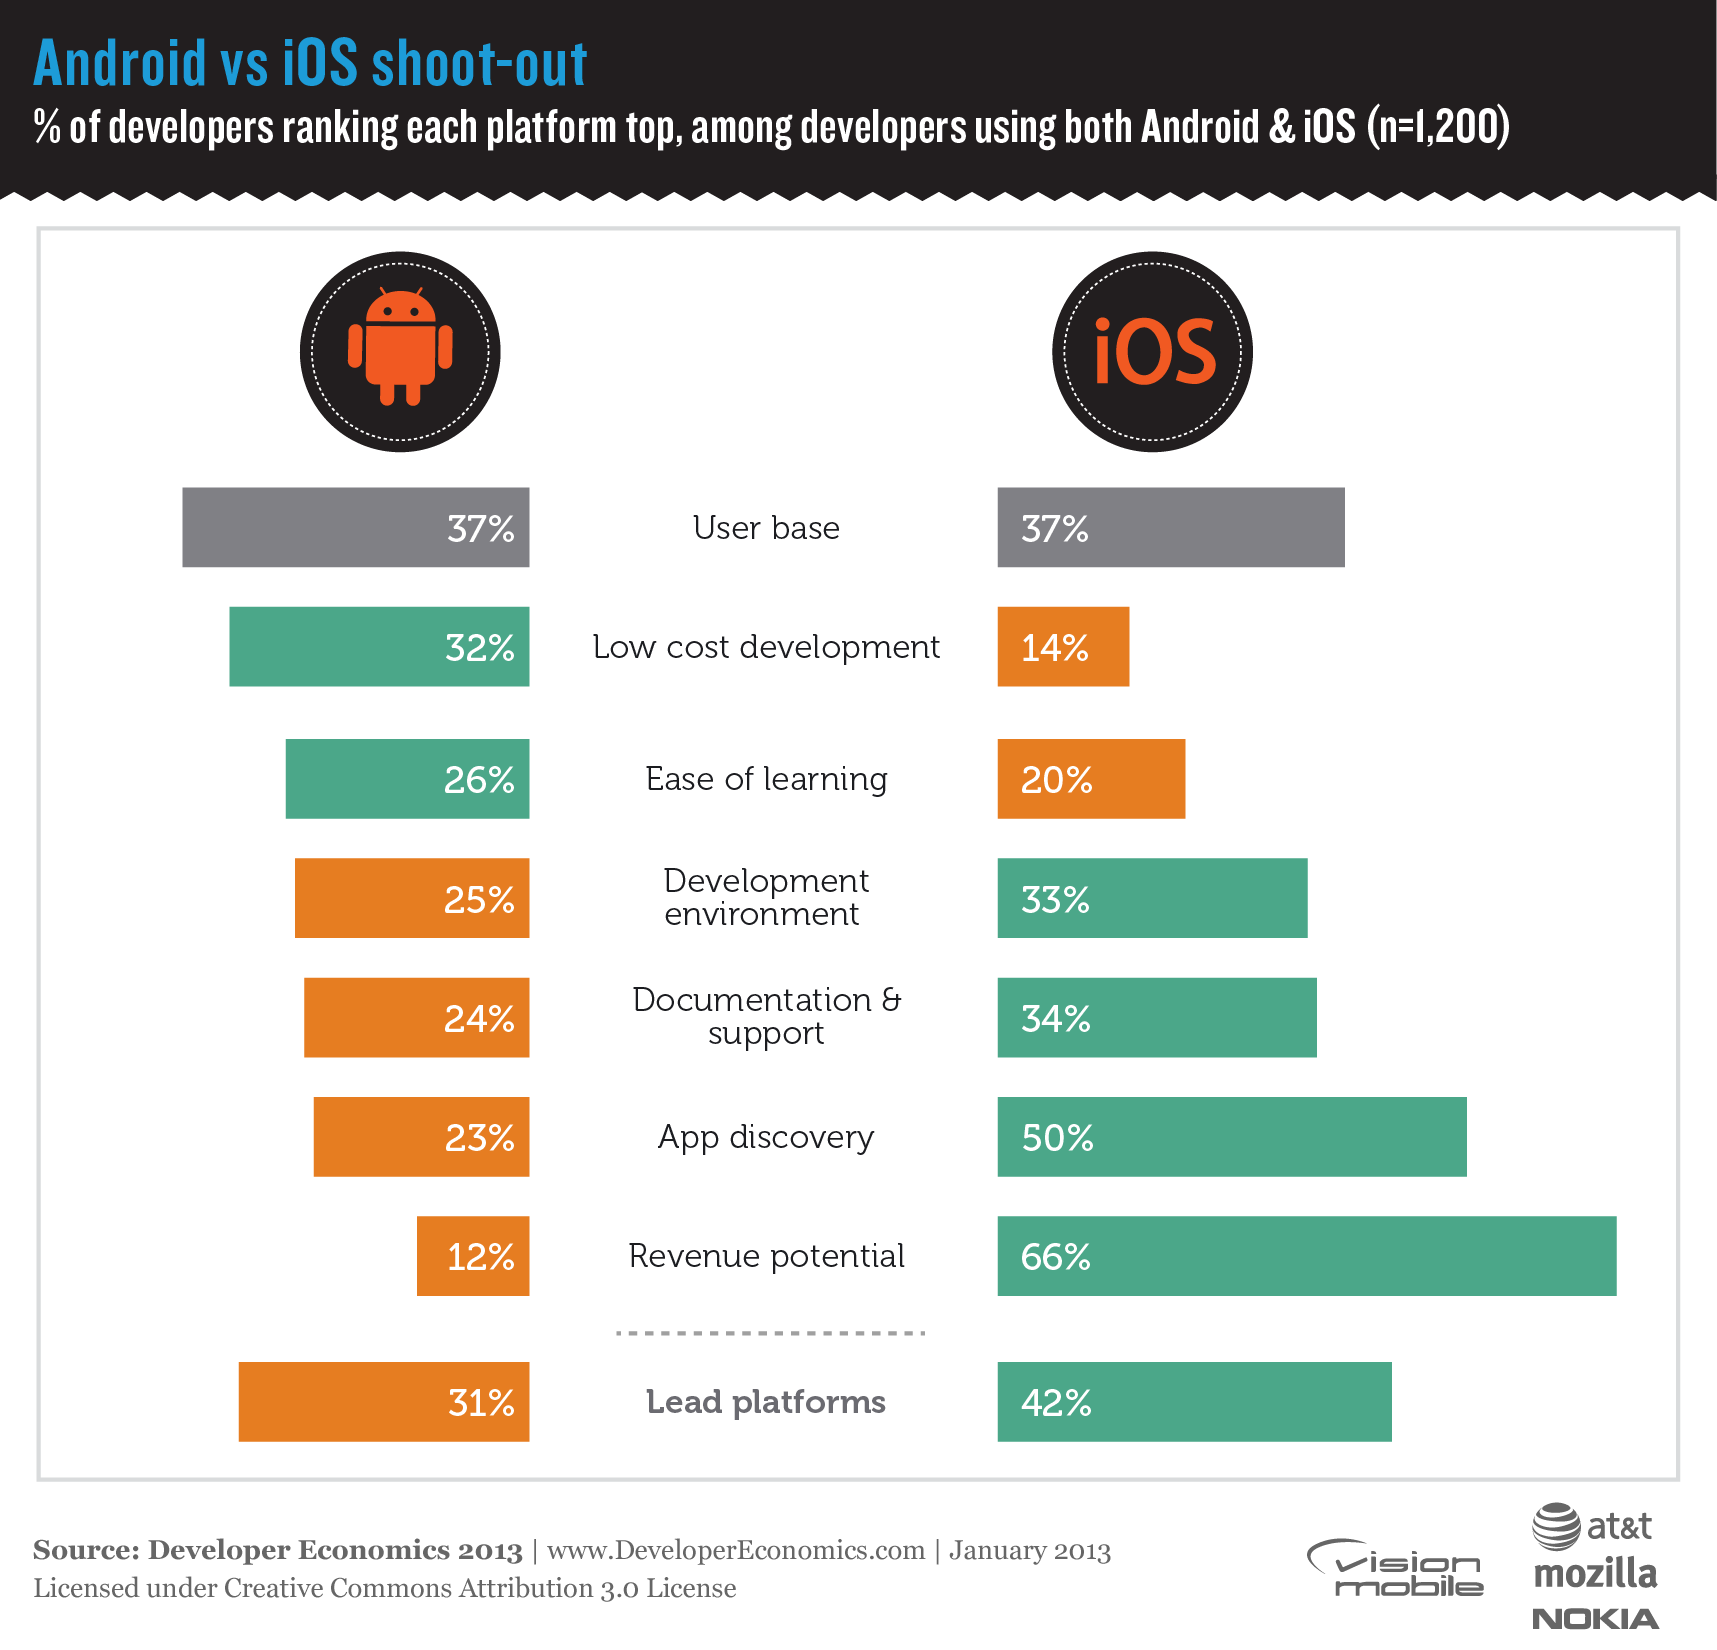
\includegraphics[width=0.8\textwidth]{Images/android_ios.png}
  \caption{Developer Economics report\cite{de} shows iOS\\as the leading platform among developers}
  \label{fig:de}
\end{figure}

As shown in Figure \ref{fig:de} iOS does indeed have a number of advantages over Android. Most importantly is the drastically increased chance of discovery as well as the expected return from applications on the iOS platform. For this project however less emphasis was placed on the success of the finished application and more on the process of creating it. Therefore the metrics of development cost and learning curve were considered to be more important. Aside from the Developer Economics findings there were a number of other more fundamental reasons as to why Android was the preferable platform. There was a certain amount of background knowledge and previous experience both with using and developing for the platform. The development environment had already been investigated and a small application developed prompting confidence in the ability to create and deploy something. Also a reasonable selection of Android devices were available for developing and testing purposes, which was favourable to using emulators and a single test device which would have been available for iOS.

The final consideration, which will be explored further in the following subsection, is that of not just overall market share but the scale of competition. IOS tends to attract the gaming market and as a result has a large selection of highly polished, top quality gaming titles. Whereas the Android market has a considerably smaller selection of games and these tend to be more basic and less graphically pleasing. Although this is changing as game developers migrate to Android it does give an advantage to new developers that might not be able to compete with the quality of iOS. 


Different versions and platforms


\subsection{Android RTS Games}


\section{Objectives}
MapWars is going to attempt to combine the the tactical aspects of these systems with a mobile experience tailored to the users surroundings. Adding in multiplayer gameplay will allow each user to interact, attack and defend against enemies as well as affect the landscape they are playing in. Taking as much of the the tactical aspects of other systems with a higher emphasise on resource gathering and long term tactical game play. Try to remove some of the fast paced ”rushing” game play that can be adopted in some \gls{rts} games. Rushing is a tactic in which a team will attack an opponent as quickly as possible as to surprise and overwhelm them. Hoping that the opponent will not have create adequate defences to counter the attack. One of MapWars main focuses in regard to strategy and game play is to have on continuous game, with many opponents. This will encourage players to concentrate on gathering resources and fortifying their base before they can have the fire-power to take on an enemies forces. As resource gathering is a major aspect of the game play, time permitting, I intend to position these resources based on real world locations. For example allowing users to gather wood or other building materials from woodland and forests that exist in the real world. Resource will deplete as users remove them but they will have a fairly short time scale in which they replenish.

\subsection{Primary Objectives}
\begin{itemize}
\item Ability to authenticate users
\item Enable players to create units, within a given range of their current location
\item Enable players to move units, within a given range of their current location
\item Display all units on a map centred on the players current location, limited to a given range
\item Units will engage with enemy that come into range
\item Location will be determined by all available sensors and the most accurate to be used
\item Appropriate portions of the application will stop functioning when minimized to preserve battery life and minimize data usage. The application should then return to a playable state when returned to
\end{itemize} 

\subsection{Expanded Objectives}
\begin{itemize}
\item Extra unit and structure types
\item Upgrade units and structures
\item Other variables such as power requirements
\item Path finding using a directions API
\item Differing mining return based on location affected by real world resources
\item Offline notifications
\end{itemize}


\subsection{Limitations \& Evaluation}
